Der Zertifizierung nach dem deutschen Eichrecht entsprechend, muss jede Ladesäule auf Eichrechtskonformität (ERK) überprüft werden.
Dieser Prozess wird immer wieder auf die gleiche Art und Weise im gleichen Umfang durchgeführt. 
Er beinhaltet somit ein entsprechendes Automatisierungspotential.

Dafür muss für jede Ladesäule ein Ladevorgang gestartet werden (Transaction), währenddessen Strom fließt und gemessen wird.   
Um die Datenintegrität der Messwerte und deren Transport sicherzustellen wird der OCPP Server verwendet. 
Mit dessen Hilfe kann nachgewiesen werden, 
dass die Daten nirgendwo in der Software geändert und ebenso unverändert an den Server übertragen und dort abgerechnet wurden. 
Nach Beenden der Transaction werden mittels einer Drittsoftware die gemessenen Daten mit den Transactiondaten verglichen.

Die gewünschte Software soll demnächst von den Mitarbeitern im End-Of-Line benutzt werden, somit muss die Bedienbarkeit der Software sehr hoch sein,
um die Fehlermöglichkeiten stark einzugrenzen und die Einarbeitungszeit zu reduzieren.

Die Anforderungen an das ERK Automatisierungstool sind:
\begin{itemize}
    \item Leichte Bedienbarkeit der Software
    \item Leicht Integrierbar in das andere Automatisierungstool
\end{itemize}

Die nachfolgende Abbildung \ref{fig:summaryDiagrammLibrary} ist ein Übersichtdiagramm der ERK Software.
\begin{figure}[H]
    \centering
    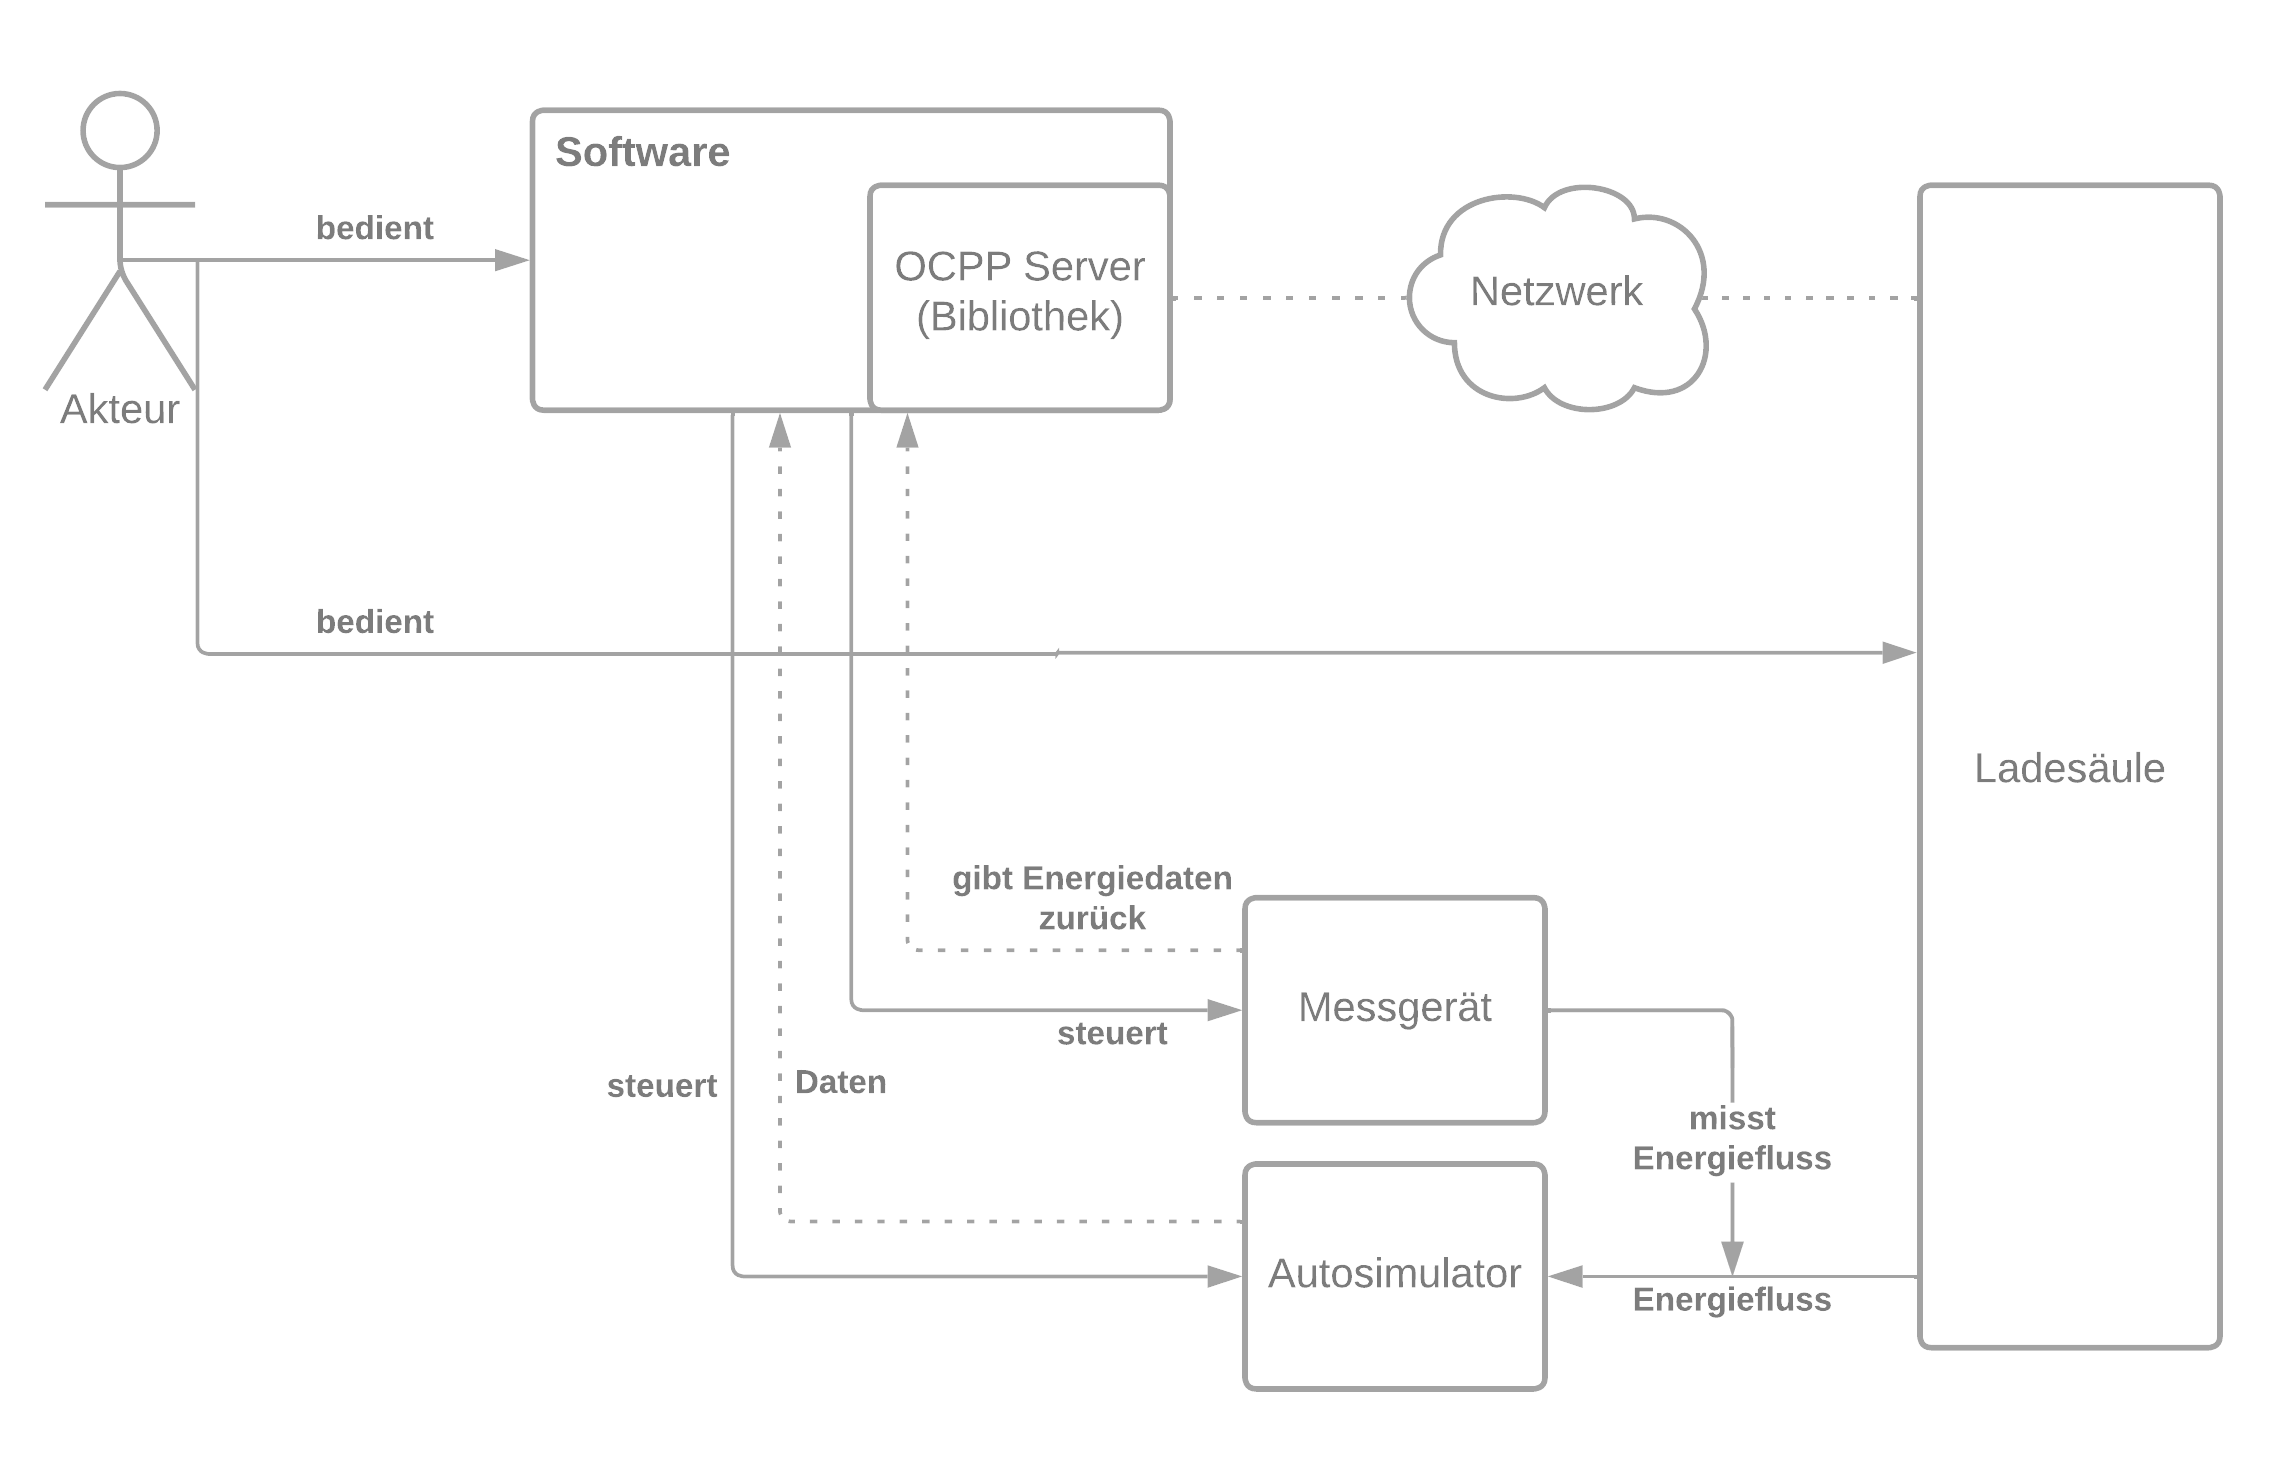
\includegraphics[width=1\textwidth]{./images/ERK.png}
    \caption[Übersichtdiagramm der ERK-Software]{Übersichtdiagramm der ERK-Software}
    \label{fig:summaryDiagrammLibrary}
\end{figure}